\section{Test 2: Rotational Dynamics---Equal Masses Precess, Entry Masses Flip}
\label{sec:dynamics}

Our second test moves from static radial equilibrium to three-dimensional rotation. Suppose a Magic Gem or radial spoke sculpture of total mass $M$ and centre of mass $\mathbf c$ is supported on a low-friction conical pivot or gimbal at the origin $O$ under uniform gravity $\mathbf g=(0,0,-g)^{\top}$ (generalizing the conical fulcrum of \texttt{weighted\_ring.stl} in \cite{mathewson2025magicgemweb}), or tossed in free space. About the pivot $O$, gravity exerts the torque
\[
\boldsymbol\tau_{\mathrm{grav}} = M\,\mathbf c \times \mathbf g,
\]
which \emph{vanishes identically in every 3D orientation if and only if the centre of mass lies at the pivot ($\mathbf c=\mathbf 0$)}. Consequently, any balanced sculpture ($\mathbf c=\mathbf 0$) supported at $O$ rotates under Earth's gravity according to Euler's exact torque-free equations \cite{arnold1989mathematical,goldstein2002classical}: in the principal body frame, the angular velocity vector $\boldsymbol\omega=(\omega_1,\omega_2,\omega_3)^{\top}$ evolves via
\begin{equation}
\label{eq:euler}
I_1\dot\omega_1 = (I_2-I_3)\omega_2\omega_3,\qquad
I_2\dot\omega_2 = (I_3-I_1)\omega_3\omega_1,\qquad
I_3\dot\omega_3 = (I_1-I_2)\omega_1\omega_2,
\end{equation}
where $I_1,I_2,I_3$ are the principal moments of inertia. For an asymmetric body with three distinct principal moments $I_1<I_2<I_3$, rotation about the intermediate axis $I_2$ is exponentially unstable: any small perturbation grows at rate $\sqrt{(I_2-I_1)(I_3-I_2)/(I_1I_3)}\,|\omega_2|$, causing the body to execute the $180^\circ$ flips of the Dzhanibekov (or tennis-racket) theorem \cite{ashbaugh1991twisting,poinsot1834theorie}.

Test~2 asks: \emph{when the $16$ unequal heights $z_{ij}$ are set spinning in $\R^3$, do their geometric inequalities produce an asymmetric top that tumbles via Dzhanibekov flips, or does line-sum equality enforce smooth axisymmetric precession?}

\subsection{Equal Masses at Unequal Heights Form a Universal Axisymmetric Rotor}

Consider first the discrete point cloud $P_S(\lambda)=\{\mathbf p_{ij}(\lambda)=(x_j,y_i,\lambda z_{ij})\}$ carrying equal point masses $m=M/N$ at the $N=n^2$ unequal lifted points (for instance, identical steel bearings mounted at the tips of the sixteen radial spokes $\mathbf p_{ij}(\lambda)$ on a lightweight hub at $O$). Because $\mathbf c=\frac1N\sum_{i,j}\mathbf p_{ij}(\lambda)=\mathbf 0$, gravitational torque about $O$ vanishes identically for every semi-magic square, and the magic line sums neutralize all off-diagonal products of inertia.

\begin{theorem}[Universal symmetric-top law, spherical-top scale, and periodic polhodes]
\label{thm:rotor}
Let $S$ be any arrangement of $\{1,\dots,n^2\}$ ($n\ge2$) whose height field has vanishing first moments $\sum_{i,j}x_jz_{ij}=\sum_{i,j}y_iz_{ij}=0$ (in particular, any semi-magic or magic square), and place equal point masses $m=M/N$ at the points $\mathbf p_{ij}(\lambda)=(x_j,y_i,\lambda z_{ij})$.
\begin{enumerate}
\item \emph{(Axisymmetric inertia tensor.)} For every $\lambda>0$, the inertia tensor about the origin $O$,
\[
I(\lambda) = \frac{M}{N}\sum_{i,j}\Bigl(\|\mathbf p_{ij}(\lambda)\|_2^2\,I_3 - \mathbf p_{ij}(\lambda)\mathbf p_{ij}(\lambda)^{\top}\Bigr),
\]
is diagonal and strictly axisymmetric about the $z$-axis:
\begin{equation}
\label{eq:inertia-point}
I(\lambda) = M\diag\bigl(I_\perp(\lambda),\, I_\perp(\lambda),\, I_{zz}\bigr),\qquad
I_\perp(\lambda) = a_n + \lambda^2 b_n,\qquad
I_{zz} = 2a_n,
\end{equation}
with universal principal inertia ratio
\begin{equation}
\label{eq:inertia-ratio}
\frac{I_\perp(\lambda)}{I_{zz}} = \frac{a_n + \lambda^2 b_n}{2a_n} = \frac{1 + \lambda^2(n^2+1)}{2}.
\end{equation}
\item \emph{(Three critical aspect ratios.)} Varying the vertical lift scale $\lambda$ drives the rotor through three regimes (\Cref{fig:precession}(a)):
\begin{enumerate}
\item At the \emph{canonical lift} $\lambda=1$,
\begin{equation}
\label{eq:ratio-lambda1}
\frac{I_\perp(1)}{I_{zz}} = \frac{n^2+2}{2},
\end{equation}
which is an exact integer for every even order $n$ ($9$ for $n=4$, $19$ for $n=6$, $33$ for $n=8$) and a half-integer for every odd order $n$ ($11/2$ for $n=3$, $27/2$ for $n=5$).
\item At the \emph{spherical-top critical scale}
\begin{equation}
\label{eq:lambda-iso}
\lambda_{\mathrm{iso}}(n) = \frac{1}{\sqrt{n^2+1}}
\qquad\Bigl(\tfrac{1}{\sqrt{10}}\approx0.3162\text{ for }n=3,\quad \tfrac{1}{\sqrt{17}}\approx0.2425\text{ for }n=4\Bigr),
\end{equation}
$I_\perp(\lambda_{\mathrm{iso}})=I_{zz}=2a_n$, so $I(\lambda_{\mathrm{iso}})=2Ma_nI_3$ is a scalar multiple of the identity: the point-weighted gem is a \emph{spherical top} for which every axis through $O$ in $\R^3$ is a principal axis of inertia.
\item At the \emph{cubic bounding-box scale} $\lambda_{\mathrm{cube}}(n)=\frac{n-1}{n^2-1}=\frac{1}{n+1}$ (where the vertical span matches the horizontal footprint $[-\frac{n-1}{2},\frac{n-1}{2}]^2$, giving $\lambda_{\mathrm{cube}}=1/5=0.20$ at $n=4$),
\begin{equation}
\label{eq:ratio-cube}
\frac{I_\perp(\lambda_{\mathrm{cube}})}{I_{zz}} = \frac{n^2+n+1}{(n+1)^2}
\qquad\Bigl(\frac{21}{25}=0.84\text{ at }n=4\Bigr).
\end{equation}
\end{enumerate}
\item \emph{(Suppression of Dzhanibekov tumbling and rational orbit closure.)} Because $I_{xx}(\lambda)=I_{yy}(\lambda)=I_\perp(\lambda)$, no distinct intermediate principal axis exists. In torque-free motion \eqref{eq:euler}, $\omega_3(t)=\omega_{3,0}$ is constant and the transverse angular velocity $(\omega_1(t),\omega_2(t))$ precesses in a uniform circle at the body-frame polhode frequency
\begin{equation}
\label{eq:polhode-freq}
\Omega_{\mathrm{body}}(\lambda) = \frac{I_\perp(\lambda)-I_{zz}}{I_\perp(\lambda)}\,\omega_{3,0}
= \frac{\lambda^2(n^2+1)-1}{\lambda^2(n^2+1)+1}\,\omega_{3,0}.
\end{equation}
At $\lambda=1$, $\Omega_{\mathrm{body}}(1)=\frac{n^2}{n^2+2}\omega_{3,0}$ is a rational multiple of the spin rate $\omega_{3,0}$, so the polhode and space-cone trajectories close periodically after $n^2+2$ spin revolutions (or $(n^2+2)/2=9$ revolutions at $n=4$). At $\lambda=\lambda_{\mathrm{iso}}(n)$, $\Omega_{\mathrm{body}}=0$ and the gem rotates steadily without wobble about any initial angular velocity vector $\boldsymbol\omega_0\in\R^3$.
\end{enumerate}
\end{theorem}

\begin{proof}
By \cite[Lem.~3.1]{mathewson2026gems}, the empirical covariance matrix $\Sigma(\lambda)=\frac1N\sum_{i,j}\mathbf p_{ij}(\lambda)\mathbf p_{ij}(\lambda)^{\top}$ has diagonal entries $\Sigma_{xx}=\Sigma_{yy}=a_n=(n^2-1)/12$ and $\Sigma_{zz}=\lambda^2b_n=\lambda^2(n^4-1)/12=\lambda^2(n^2+1)a_n$, while $\Sigma_{xy}=0$ by grid symmetry and $\Sigma_{xz}=\Sigma_{yz}=0$ by vanishing of the first moments. Since $I(\lambda)=M\bigl(\tr(\Sigma(\lambda))I_3-\Sigma(\lambda)\bigr)$, we obtain \eqref{eq:inertia-point} and \eqref{eq:inertia-ratio}. Specializing \eqref{eq:inertia-ratio} to $\lambda=1$, $\lambda=(n^2+1)^{-1/2}$, and $\lambda=(n+1)^{-1}$ yields (2a)--(2c). Substituting $I_1=I_2=I_\perp(\lambda)$ and $I_3=I_{zz}$ into Euler's equations \eqref{eq:euler} gives $\dot\omega_3=0$ and $\dot\omega_1=\Omega_{\mathrm{body}}\omega_2$, $\dot\omega_2=-\Omega_{\mathrm{body}}\omega_1$ with $\Omega_{\mathrm{body}}$ as in \eqref{eq:polhode-freq}.
\end{proof}

\begin{figure}[htbp]
\centering
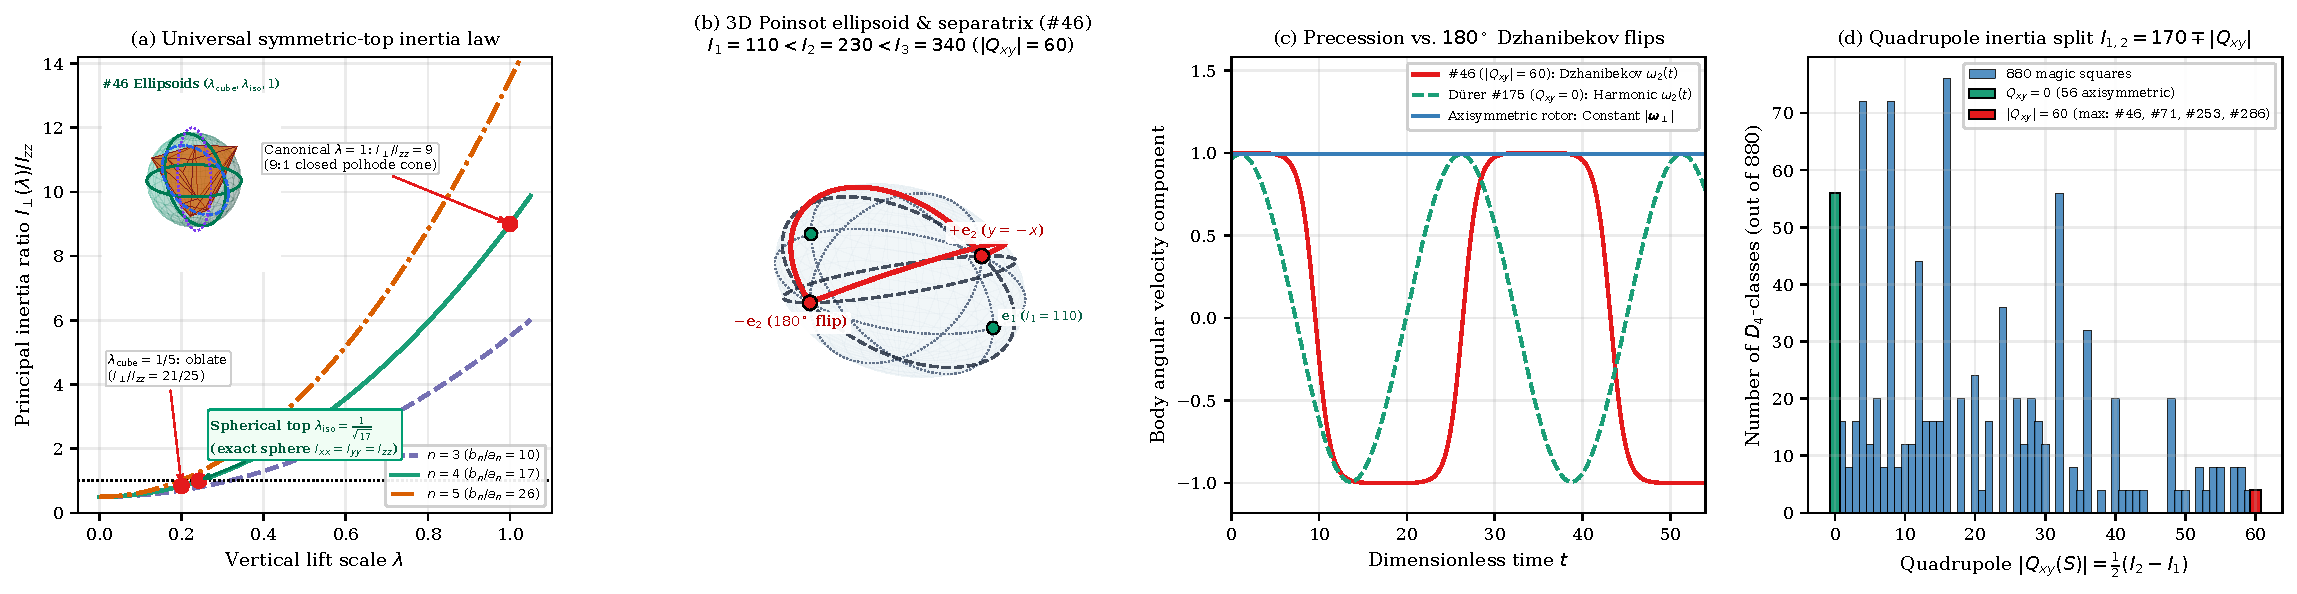
\includegraphics[width=\textwidth]{figures/fig_precession_dynamics.pdf}
\caption{Three-dimensional rotational dynamics of Magic Gems. (a)~Universal principal inertia ratio $I_\perp(\lambda)/I_{zz}=\frac12(1+\lambda^2(n^2+1))$ versus vertical scale $\lambda$ for orders $n=3,4,5$, with 3D inertia ellipsoids at the cubic 3D-print scale $\lambda_{\mathrm{cube}}=1/5$ ($21/25$), the isotropic spherical-top transition $\lambda_{\mathrm{iso}}=1/\sqrt{17}$ ($1$), and the canonical lift $\lambda=1$ ($9$) for $n=4$. (b)~Triaxial Poinsot energy ellipsoid $\frac12\sum I_k\omega_k^2=E$ of entry-weighted square \#46 ($I_1=110<I_2=230<I_3=340$), showing the figure-eight separatrix through the unstable intermediate saddle $\pm\boldsymbol\omega_2$ and the heteroclinic polhode orbit connecting $+\omega_2$ to $-\omega_2$. (c)~Time series of Euler's equations \eqref{eq:euler}: an axisymmetric magic rotor (D\"urer \#175 or any point-weighted gem) precesses harmonically with constant $|\boldsymbol\omega_\perp|$, whereas entry-weighted square \#46 ($|Q_{xy}|=60$) undergoes periodic $180^\circ$ Dzhanibekov flips $\omega_2(t)\in[+1,-1]$ about its intermediate diagonal axis. (d)~Census of the quadrupole moment $|Q_{xy}(S)|=|\sum z_{ij}x_jy_i|=\frac12(I_2-I_1)$ across the $880$ order-four magic squares.}
\label{fig:precession}
\end{figure}

\subsection{Unequal Entry Masses Expose \texorpdfstring{$Q_{xy}$}{Qxy} and Trigger Dzhanibekov Flips}

What breaks the universal axisymmetric rotation of \Cref{thm:rotor}? Weighting each cell by its \emph{unequal magic entry} $m_{ij}=s_{ij}$ (as in the planar balancing wheel \texttt{weighted\_ring.stl} \cite{mathewson2025magicgemweb}). While Loly's theorem \cite{loly2004invariance} keeps the diagonal moments equal ($I_{xx}=I_{yy}=I_0$), the unequal masses expose a second-order quadrant inequality—the planar quadrupole moment $Q_{xy}(S)=\sum_{i,j}z_{ij}x_jy_i$—together with the cubic 3D vector resultant $\mathbf V_3(S;\lambda)$ from Test~1. On square \#46 (\Cref{fig:hero-squares}(d)), for example, the heavy entries $\{16,13,15,14\}$ concentrate in the NW/SE quadrants ($xy<0$) while the light entries $\{1,4,2,3\}$ sit in the NE/SW quadrants ($xy>0$). Flicking the board to spin about its intermediate diagonal axis $y=-x$ ($I_2=230$) places the angular velocity directly on the saddle of the Poinsot energy ellipsoid (\Cref{fig:precession}(b)), triggering a $180^\circ$ Dzhanibekov flip (\Cref{fig:precession}(c)).

\begin{theorem}[Entry-weighted inertia split, quadrupole Dzhanibekov instability, and 3D lifted tensor]
\label{thm:quadrupole-split}
Let $S$ be any semi-magic square of order $n$, and assign entry masses $m_{ij}=s_{ij}=\bar s+z_{ij}$ with total mass $M=\sum_{i,j}s_{ij}=N\bar s=n^2(n^2+1)/2$.
\begin{enumerate}
\item \emph{(Planar inertia tensor and diagonal principal axes.)} When the masses $m_{ij}=s_{ij}$ are placed at the planar grid positions $(x_j,y_i,0)\in\R^3$, the centre of mass lies at $O$ and the $3\times3$ inertia tensor about $O$ is
\begin{equation}
\label{eq:inertia-entry}
I^{(s)}(S) = \begin{pmatrix}
I_0 & -Q_{xy}(S) & 0\\
-Q_{xy}(S) & I_0 & 0\\
0 & 0 & 2I_0
\end{pmatrix},\quad
I_0 = M a_n = \frac{n^2(n^4-1)}{24},\quad
Q_{xy}(S) = \sum_{i,j}z_{ij}x_jy_i.
\end{equation}
Its principal moments of inertia are
\begin{equation}
\label{eq:principal-entry}
I_1(S) = I_0 - |Q_{xy}(S)|,\qquad
I_2(S) = I_0 + |Q_{xy}(S)|,\qquad
I_3 = 2I_0,
\end{equation}
with horizontal principal axes directed along the two main diagonals $y=\pm x$.
\item \emph{(Order-four Dzhanibekov dichotomy.)} At order $n=4$, $I_0=170$ and $I_3=340$. Across the $880$ magic squares of order~$4$ (\Cref{fig:precession}(b--d)):
\begin{enumerate}
\item Exactly $56$ squares satisfy $Q_{xy}(S)=0$ ($48$ associative squares in Group~III, including D\"urer's \#175, plus $8$ in Groups~IX--X), remaining axisymmetric rotors with $I_1=I_2=170$.
\item The remaining $824$ squares have $|Q_{xy}(S)|\in\{1,\dots,60\}$ (peaking at $|Q_{xy}|=60$, $I_1=110 < I_2=230 < I_3=340$, on Group~VI squares \#46, \#71, \#253, and \#286), and undergo unstable Dzhanibekov flips about $y=-\operatorname{sgn}(Q_{xy})\,x$ at dimensionless exponential growth rate
\[
\Gamma(S) = \sqrt{\frac{(I_2-I_1)(I_3-I_2)}{I_1 I_3}} = \sqrt{\frac{|Q_{xy}(S)|}{I_0}} = \sqrt{\frac{|Q_{xy}(S)|}{170}}.
\]
\end{enumerate}
\item \emph{(3D lifted entry-weighted gem and unification with $\mathbf V_3(S;\lambda)$.)} When the entry masses $m_{ij}=s_{ij}$ are placed at the 3D lifted points $\mathbf p_{ij}(\lambda)=(x_j,y_i,\lambda z_{ij})$ ($\lambda>0$), the centre of mass shifts vertically to $\mathbf c^{(s)}(\lambda)=(0,0,z_{\mathrm{cm}}(\lambda))$ with $z_{\mathrm{cm}}(\lambda)=\lambda b_n/\bar s=\frac{\lambda(n^2-1)}{6}$ ($=\frac52\lambda$ at $n=4$). Because $\sum_{i,j}z_{ij}^3=0$, the diagonal moments of inertia about $O$ are $I_{xx,O}^{(s)}(\lambda)=I_{yy,O}^{(s)}(\lambda)=M(a_n+\lambda^2 b_n)$ and $I_{zz,O}^{(s)}(\lambda)=2I_0$, matching the equal-mass gem in \Cref{thm:rotor}(1). Translating to the true centre of mass $\mathbf c^{(s)}(\lambda)$ via Steiner's parallel-axis theorem leaves $I_{zz,\mathrm{cm}}^{(s)}=2I_0$ and all off-diagonal products unchanged while subtracting $Mz_{\mathrm{cm}}(\lambda)^2$ from the horizontal diagonal moments:
\[
I_{xx,\mathrm{cm}}^{(s)}(\lambda) = I_{yy,\mathrm{cm}}^{(s)}(\lambda)
= M\!\left(a_n + \lambda^2 b_n\!\left(1 - \frac{b_n}{\bar s^2}\right)\right)
= M a_n\!\left(1 + \frac{2(n^2+2)}{3}\lambda^2\right)
\]
($=170(1+12\lambda^2)$ at $n=4$). In both frames ($O$ and $\mathbf c^{(s)}(\lambda)$), the off-diagonal products of inertia are $I_{xy}^{(s)}=-Q_{xy}(S)$ and
\[
\bigl(I_{xz}^{(s)}(\lambda),\, I_{yz}^{(s)}(\lambda)\bigr)
= -\lambda\sum_{i,j}z_{ij}^2(x_j,y_i)
= -\lambda^{-1}\Bigl(\bigl(\mathbf V_3(S;\lambda)\bigr)_x,\, \bigl(\mathbf V_3(S;\lambda)\bigr)_y\Bigr).
\]
Consequently, an order-four magic square has a diagonal, axisymmetric 3D entry-weighted inertia tensor if and only if it is one of the $48$ associative squares ($Q_{xy}=0$ and $\mathbf V_3=\mathbf 0$).
\end{enumerate}
\end{theorem}

\begin{proof}
(1)--(2) Since every row excess $R_i=\sum_jz_{ij}$ and column excess $C_j=\sum_iz_{ij}$ vanishes, $\sum_{i,j}s_{ij}x_j^2=\bar s\sum_{i,j}x_j^2+\sum_jx_j^2C_j=M a_n=I_0$ and $\sum_{i,j}s_{ij}y_i^2=I_0$, giving $I_{xx}=I_{yy}=I_0$ and $I_{zz}=2I_0$. Since $\sum_{i,j}x_jy_i=0$, $I_{xy}=-\sum_{i,j}s_{ij}x_jy_i=-Q_{xy}(S)$. Diagonalizing $\bigl(\begin{smallmatrix}I_0 & -Q_{xy}\\ -Q_{xy} & I_0\end{smallmatrix}\bigr)$ yields eigenvalues $I_0\mp|Q_{xy}|$ along $(1,\pm1)/\sqrt{2}$, proving \eqref{eq:inertia-entry}--\eqref{eq:principal-entry}. At $n=4$, $I_0=170$, $|Q_{xy}|\le 60 < 170$, and $I_3-I_2=2I_0-(I_0+|Q_{xy}|)=I_1$ simplifies $\sqrt{(I_2-I_1)(I_3-I_2)/(I_1I_3)}$ to $\sqrt{|Q_{xy}|/I_0}$.

(3) At $\mathbf p_{ij}(\lambda)$, $\sum_{i,j}s_{ij}(x_j,y_i)=\mathbf 0$ while $\sum_{i,j}(\bar s+z_{ij})\lambda z_{ij}=\lambda\sum_{i,j}z_{ij}^2=N\lambda b_n$, giving $z_{\mathrm{cm}}(\lambda)=\lambda b_n/\bar s$. Since $\sum_{i,j}z_{ij}^3=0$, $\sum_{i,j}(\bar s+z_{ij})\lambda^2z_{ij}^2=M\lambda^2b_n$, so $I_{xx,O}^{(s)}(\lambda)=I_{yy,O}^{(s)}(\lambda)=M(a_n+\lambda^2b_n)$. Steiner's theorem subtracts $Mz_{\mathrm{cm}}(\lambda)^2\diag(1,1,0)$, and $1-b_n/\bar s^2=\frac{2(n^2+2)}{3(n^2+1)}$ gives $b_n(1-b_n/\bar s^2)=\frac{2(n^2+2)}{3}a_n$. Finally, $I_{xz}^{(s)}(\lambda)=-\lambda\sum_{i,j}z_{ij}^2x_j=-\lambda^{-1}(\mathbf V_3)_x$ and similarly for $I_{yz}^{(s)}(\lambda)$, both of which vanish alongside $Q_{xy}(S)$ on all $48$ associative squares by \Cref{thm:3d-power}(1).
\end{proof}

\subsection{From Point Clouds to Continuous Polyhedra: Why Solid Hulls Tilt on the Pivot}

What happens to rotational stability when we replace the discrete point cloud $P_S$ by the uniform-density 3D solid polyhedron $\mathcal G_0(S)=\conv P_S$? Decomposing $\mathcal G_0(S)$ into exact rational tetrahedra (\Cref{sec:appendix}) shows that about its own centre of mass $\mathbf c_0(S)$, the solid inertia tensor remains remarkably close to the axisymmetric point-mass rotor of \Cref{thm:rotor}: across all $880$ squares at $\lambda=1$, the ratio of the mean transverse moment $\frac12(I_2+I_3)$ to the axial moment $I_1$ averages $9.41$ (range $[7.34,\,11.57]$, tracking the point-mass value $9$), and the relative transverse splitting remains below $2.5\%$ ($\frac{I_3-I_2}{I_2}\in[0.00004,\,0.0243]$, mean $0.0071$).

Yet when we place the cast solid $\mathcal G_0(S)$ on our pivot at the grid origin $O$ under gravity, a more basic failure occurs: on $829$ of the $880$ squares, taking the convex hull shifts the solid centre of mass $\mathbf c_0(S)$ off the origin ($\mathbf c_0(S)\ne\mathbf 0$), so gravity immediately exerts a tipping torque $\boldsymbol\tau_{\mathrm{grav}}=M\mathbf c_0(S)\times\mathbf g\ne\mathbf 0$. Understanding why the convex hull breaks centroid balance—and how the interior points of the magic square restore it—is the subject of Test~3.
